\begin{satz}[lokale Darstellung einer Mannigfaltigkeit als Graph]
\mbox{} \\
$M \subset \mathbb{R}^{n}$ ist genau dann eine d-dimensionale $C^{q}$-Mannigfaltigkeit, wenn für alle $u\in M\subset\mathbb{R}^n$ eine Umgebung $U$ von $u$ bezüglich $M$ und eine offene Menge $W\subset\mathbb{R}^d$ existiert, sodass (gegebenefalls unter einer Koordinatenpermutation $\pi$ im $\mathbb{R}^n$) für mindenstens ein $f \in C^q (W, \mathbb{R}^{n-d})$ ein $\psi$ mit $\psi[W]=U$ existiert, das
\begin{equation*}
\psi(v)\coloneqq\pi(v,f(v)) \ \ \ \ \forall v\in W
\end{equation*}
erfüllt. (d.h. $U=\graph f$)

\end{satz}

Wir können also sagen, dass sich jede $C^q$-Mannigfaltigkeit \emph{lokal} als Graph einer $C^q$-Funktion darstellen lassen können muss. Die Umkehrung ist genauso richtig. So ist also jeder Graph einer $C^q$-Funktion gleichzeitig Mannigfaltigkeit.

\begin{proof}

Die Rückrichtung folgt direkt aus den Beispielen 2 und 4. Für die Hinrichtung fixieren wir ein $\tilde{u} \in M $ und wählen $\varphi : \tilde{V} \in \mathbb{R}^d
\rightarrow \tilde{U} \subset \mathbb{R}^n $ als zugehörige Parametrisierung von $\tilde{u} = \varphi (\tilde{x})$. Wir schreiben nun $\varphi$ als 
\begin{equation*}
\varphi(x)=\begin{pmatrix}\varphi_I(x) \in\mathbb{R}^d \\ \varphi_{II}(x) \ \in\mathbb{R}^{n-d} \end{pmatrix}
\end{equation*}

Da $\varphi'$ regulär sein muss, folgt (mit eventueller Vertauschung $\pi$ der Zeilen), dass auch $\varphi_I'(\tilde{x})\in\mathbb{R}^{d\times d}$ regulär ist. Zerlegen wir nun $\tilde{u}=\pi(\tilde{u},\tilde{w})$ mit $v\in\mathbb{R}^d$,

\begin{center}
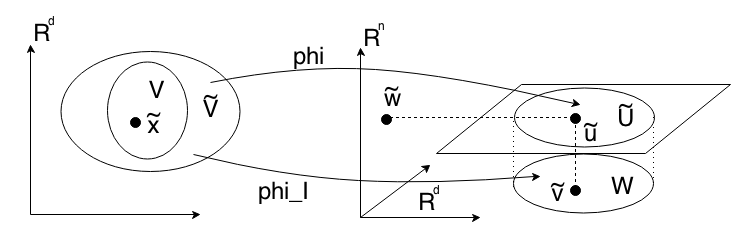
\includegraphics[scale=0.5]{pictures/MA2_0010}\\
\end{center}

so folgt aus dem \emph{Satz über inverse Funktionen}, dass es ein offenes $V\subset\tilde{V}$ gibt, in dem ein $\tilde{x}\in V$ liegt und wiederum ein $W\subset\mathbb{R}^d$, in dem ein $\tilde{v}\in W$ liegt, so dass $\tilde{v}$ durch $\varphi^{-1}$ auf $\tilde{x}$ abgebildet wird. $\varphi^{-1}$ exisitert auf jeden Fall, da $\varphi$ homöomorph und $C^q$-differenzierbar ist. Es ist also

\begin{equation*}
\varphi_I^{-1}(\tilde{v})=\tilde{x}
\end{equation*}

Wählen wir nun 

\begin{equation*}
f(v) \coloneqq \varphi_{II} \left(\varphi_I ^{-1} (v)\right)
\end{equation*}
\linebreak
welches für alle $v \in W $ $q$-mal stetig differenzierbar ist, also in $C^q \left(W, \mathbb{R}^{n-d}\right) $ liegt, und setzen 

\begin{equation*}
\psi (v) \coloneqq \varphi \left(\varphi_I ^{-1} (v) \right) =
\left( \varphi_I \left(\varphi_I ^{-1} (v),\right( 
\varphi_{II} \left(\varphi_I ^ {-1} (v) \right) \right) = \pi \left(v, f(v)\right)
\end{equation*}
\linebreak
So folgt unmittelbar, dass $\psi (\tilde{v}) = \pi (\tilde{v}, \tilde{w}) = \tilde{u}$ ist und $\psi (w) = \varphi (v)$ in $M$ liegt. Aufgrund der Homöomorphie von $\varphi : \tilde{V} \rightarrow \tilde{U} $ ist $\varphi[V]$ offen in $M$ und somit auch $U\coloneqq\psi(W)$ offen bezüglich $M$. Da $U$ nun eine Umgebung von $\tilde{u}$ bezüglich $M$ ist und $\tilde{u}$ beliebig war, folgt direkt die Behauptung.
\end{proof}

\begin{satz}[Charakterisierung von Mannigfaltigkeiten mit umgebendem Raum]
\mbox{} \\
$M \subset \mathbb{R}^{n}$ ist genau dann eine d-dimensionale $C^{q}$-Mannigfaltigkeit, wenn für alle $u\in M$ eine Umgebung $\tilde{U}$ bezüglich des $\mathbb{R}^n$ exisitert, sodass $\psi:\tilde{U}\rightarrow\tilde{V}$ (mit $V\subset\mathbb{R}^n$ offen) ein $C^q$-Diffeomorphismus ist und
    \begin{equation*}
    \psi \left( \tilde{U} \cap M \right) =
    \tilde{V} \cap \left( \mathbb{R}^d \times {0} \right) 
    \end{equation*}
erfüllt.
\begin{center}
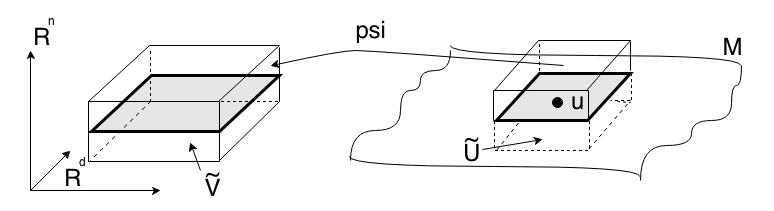
\includegraphics[scale=0.5]{pictures/MA2_0011}\\
\end{center}
\end{satz}

Dies ist eine Charakterisierung, die den umgebenden Raum nutzt und oft auch als Definition von $C^q$-Mannigfaltigkeiten verwendet wird.
    
\begin{proof}
Für die Rückrichtung schränken wir $\psi $ auf $\tilde{U} \cap M $ und erhalten sofort Karten, was die Behauptung bestätigt. Für die Hinrichtung fixieren wir ein $\tilde{u} \in M $ und wählen wieder $\tilde{U} \subset M $, $W \subset \mathbb{R}^d $ und ein $f \in C^q \left( W, \mathbb{R}^{n-d} \right)$. Gemäß Satz 29.1 setzen wir o.B.d.A $\pi = $ \textit{id} und zerlegen $\tilde{u} = \left( \tilde{v}, f \left( \tilde{v} \right) \right) \in \mathbb{R}^d \times \mathbb{R}^{n-d}$. Nun sei $\hat{U} \coloneqq W \times \mathbb{R}^{n-d} \eqqcolon \hat{V} $, welches den \emph{Zylinder} aus $U$ und $W$ in Beweis zu Satz 29.1 liefert.
Setzen wir schließlich noch $\tilde{\varphi}: \hat{V} \rightarrow \hat{U} $ mit
\begin{equation*}
\tilde{\varphi} (v,w) \coloneqq (v, f(v) + w)
\end{equation*}
welches offenbar $\in C^q$ ist und erhalten, dass
\begin{equation*}
\tilde{\varphi}' \left( \tilde{v}, 0 \right) =
    \begin{pmatrix}
    \textit{id}_d & 0 \\
    f'(v)         & \textit{id}_{n-d}
    \end{pmatrix}
\end{equation*}
regulär ist. Nach dem \emph{Satz ü. inverse Funktionen} exisitert wiederum eine Umgebung $ \tilde{U} \subset \hat{U}$ von $\tilde{u}$ und eine Umgebung $ \tilde{V} \subset \hat{V} $ von $ \left( \tilde{v}, 0 \right) $, sodass $\tilde{\psi} \coloneqq \tilde{\varphi}^{-1} \in C^q \left( \tilde{U}, \tilde{V} \right) $
exisitiert. Wegen $\tilde{\varphi} \left( \tilde{V} \cap \left( \mathbb{R}^d \times {0} \right) \right)
= \tilde{U} \cap M $ folgt die Behauptung.
\end{proof}

\begin{folgerung}
Sei $M \subset \mathbb{R}^n$ eine d-dimensionale $C^q$-Mannigfaltigkeit und $\varphi: V \subset \mathbb{R}^d \rightarrow U \subset M $ die Parametrisierung um $u \in M $. Dann gibt es die offenen Mengen $\tilde{U}, \tilde{V} \subset \mathbb{R}^n $ mit $ U \subset \tilde{U}, V \times {0} \subset \tilde{V} $ für die $\tilde{\varphi} : \tilde{V} \rightarrow \tilde{U} $ abbildet, ein $C^q$-Diffeomorphismus ist und $\tilde{\varphi} (x, 0) = \varphi (x) \forall x \in V $
\end{folgerung}

\begin{proof}
Folgt aus Beweisen von Satz 29.1 und 29.2
\end{proof}

\begin{satz}[lokale Darstellung von Mf als Niveaumenge]
\mbox{} \\
$M \subset \mathbb{R}^n $ sei d-dimensionale $C^q$-Mannigfaltigkeit. \\
$\Longleftrightarrow \forall u \in M $ existiert eine Umgebing $\tilde{U}$ von $u$
bezüglich $\mathbb{R}^n$ und \\
$f \in C^q \left( \tilde{U}, \mathbb{R}^{n-d} \right)$ 
mit $\textit{rang } f' (u) = n-d $ und \\
$\tilde{U} \cap M = \left\lbrace \tilde{u} \in \tilde{U} | f (\tilde{u}) = 0 \right\rbrace $
\end{satz}

\textbf{somit:} $M$ ist eine $C^q$-Mannigfaltigkeit genau dann, 
wenn $M$ die lokale Niveaumenge einer $C^q$-Funktion $f$ ist. \\

\textbf{Bemerkung:} $c \in \mathbb{R}^{n-d} $ heißt \textit{regulärer Wert} von
$f \in C^q \left( \tilde{U}, \mathbb{R}^{n-d} \right) $, \\
$\tilde{U} \subset \mathbb{R}^n $
offen, falls $\textit{rang } f' (u) = n-d \forall u \in \tilde{U} $ mit $f(u) = c $ \\
Folglich ist $M \coloneqq \left\lbrace u \in \tilde{U} | f(u) = c \right\rbrace $ 
eine d-dimensionale $C^q$-Mannigfaltigkeit, falls $c$ ein regulärer Wert von $f$ ist.

\begin{proof}
$"\Leftarrow":$ gemäß Bsp. 5 erhält man lokale Parametriesierung \\
$\Rightarrow$ Behauptung. \\
$"\Rightarrow":$ fixiere $\tilde{u} \in M$, 
wähle $\tilde{U}, \tilde{V} \subset \mathbb{R}^n, 
\tilde{\psi}: \tilde{U} \rightarrow \tilde{V} $ gemäß Satz 29.2 \\
sei $f \coloneqq \left( \tilde{\psi}_{d+1}, \ldots , \tilde{\psi}_n \right)$,
offenbar $f \in C^q \left(  \tilde{U}, \mathbb{R}^{n-d} \right) $ \\
mit $\tilde{\psi}$ aus dem Beweis zu Satz 29.2:
$\tilde{\psi}' (\tilde{u}) = \tilde{\varphi}' (\tilde{v}, 0)^{-1} $ ist regulär \\
$\Rightarrow f'(\tilde{u}) $ hat vollen Rang, d.h. $\textit{rang } f'(\tilde{u}) = n-d $ \\
nach Konstruktion $ \left\lbrace u \in \tilde{U} | f(u) = 0 \right\rbrace = U \cap M
\Rightarrow $ Behauptung.
\end{proof}

\begin{lemma}[Kartenwechsel] 
\mbox{} \\
Sei $M \in \mathbb{R}^n $ d-dimensionale Mannigfaltigkeit \\
und $\varphi_1^{-1}, \varphi_2^{-1} $ Karten mit zugehörigem Kartengebiet 
$U_1 \cap U_2 \neq \emptyset $ \\
$\Longrightarrow 
\varphi_2^{-1} \circ \varphi_1 : \varphi_1^{-1} \left( U_1 \cap U_2 \right)
\rightarrow \varphi_2^{-1} \left( U_1 \cap U_2 \right) $ ist $C^q$-Diffeomorphismus.\\
\begin{center}
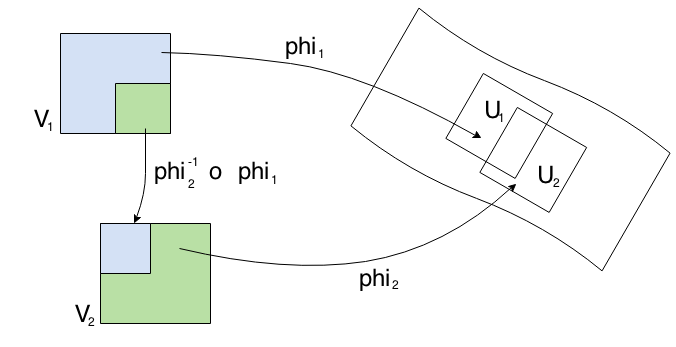
\includegraphics[scale=0.5]{pictures/MA2_0012}\\
\end{center}
\end{lemma}

\begin{proof}
Ersetze $\varphi_1, \varphi_2 $ mit $\tilde{\varphi}_1, \tilde{\varphi}_2 $
gemäß Folgerung 29.3 \\
$\Rightarrow$ Einschränkung von $\tilde{\varphi}_2^{-1} \circ \tilde{\varphi}_1 $
liefert Behauptung. 
\end{proof}

\begin{definition}
Sei $M \subset \mathbb{R}^n $ d-dimensionale Mannigfaltigkeit. \\
Ein Vektor $v \in \mathbb{R}^n $ heißt \textbf{Tangentialvektor} in $u \in M $ an $M$, \\
falls eine stetig differenzierbare Kurve 
$\gamma: (-\delta, \delta) \rightarrow M (\delta > 0) $ exisitiert mit \\
$\gamma (0) = u $ und $\gamma' (0) = v $. \\
Die Menge aller Tangentialvektoren $T_uM$ heißt Tangentialraum.\\
\begin{center}
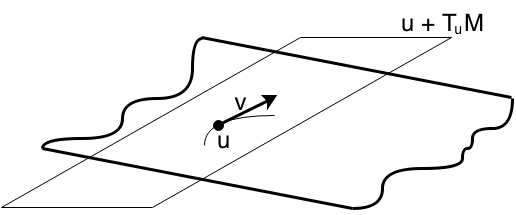
\includegraphics[scale=0.5]{pictures/MA2_0013}\\
\end{center}
\end{definition}

\begin{satz}
Sei $M \in \mathbb{R}^n $ eine d-dimensionale Mannigfaltigkeit, \\
$u \in M $, $ \varphi : V \rightarrow U $ der zugehörige Parameter um $u$ \\
$\Longrightarrow T_uM $ ist d-dimensionaler $( \mathbb{R}-) $ Vektorraum und \\
    \begin{equation}
    T_uM = \underbrace{\varphi'(x)}_{L \left( \mathbb{R}^d, \mathbb{R}^n \right) }
    \left( \mathbb{R}^d \right) \text{ für } x = \varphi^{-1} (u) 
    \end{equation}
wobei $T_uM$ unabhängig vom speziellen Parameter $\varphi$ ist.
\end{satz}

\begin{proof}
Sei $\gamma: (-\delta, \delta) \rightarrow M eine C^1$-Kurve mit $\gamma(0) = u $ \\
$\Rightarrow g \coloneqq \varphi^{-1} \circ \gamma $ ist $C^1$-Kurve, 
$g: (-\delta, \delta) \rightarrow \mathbb{R}^d $ mit $ g(0) = x $ und
    \begin{equation*}
    \gamma' (0) = \varphi' (x) g'(0) \text{, } \varphi' (x) \text{ist regulär.}
    \tag{$\ast$}
    \end{equation*}
Offenb. liefert auch jede $C^1$-Kurve $g$ in $\mathbb{R}^d $ durch $x$
eine $C^1$-Kurve $\gamma$ in $M$ mit $(\ast)$ \\
Die Menge aller Tangentialvektoren $g'(0)$ von $C^1$-Kurven $g$ in $\mathbb{R}^d $
ist offenbar $\mathbb{R}^d $ \\
$\Rightarrow $ 
29.4 $ \xRightarrow{\varphi' (x) \text{ ist regulär}} \textit{dim } T_uM = d $ \\
da $(\ast)$ für jeden Parameter $\varphi$ gilt, ist $T_uM$ unabhängig von $\varphi$.
\end{proof}

\textbf{Bemerkung:}
Man bezeichnet auch $(u, T_uM) \subset M \times \mathbb{R}^n$
als Tangentialraum und
$TM = \bigcup\limits_{U \in M} (u, T_uM) \subset M \times \mathbb{R}^n $
als Tangentialbündel.

\begin{beispiel}
Sei $M \subset \mathbb{R}^n $ offen  \\
$\Rightarrow $ $M$ ist ist n-dimensionale Mannigfaltigkeit und 
$T_uM = \mathbb{R}^n \forall u \in M $
\end{beispiel}

\begin{definition}
Sei $M \subset \mathbb{R}^n $ d-dimensinale Mannigfaltigkeit. \\
Ein Vektor $w \in \mathbb{R}^n $ heißt \textbf{Normalenvektor} in $u \in M $ an $M$, falls\\
$\langle w,v \rangle = 0 \forall v \in T_uM $
(d.h. $w \bot v \forall v \in T_uM$) \\
Die Menge aller Normalenvektoren $N_uM = T_uM^{\bot} $ heißt \\
\textbf{Normalenraum} von $M$ in $u$. 
\end{definition}